% soctepmlate unofficial - SOČ = Středoškolská odborná činnost - Czech competition
% Author: Vojtěch Boček
% Edit by: Jaroslav Páral
% Version: 2018-02-12
% Source code: https://github.com/RoboticsBrno/soctemplate/
% Base on: http://www.jcmm.cz/cz/sablona-soc.html
% License: CC BY 4.0
% Edited by: Pavel Šrytr for his SOC team needs and to meets the requierements of the SOC supervisor
% Further edited by Jakub Hampl


\documentclass{socthesis}

\usepackage{subcaption}
\usepackage{amsmath}
\usepackage{enumitem}
\usepackage[T1]{fontenc}
\usepackage{hyperref}
\usepackage{siunitx}
\usepackage{float}
\usepackage{titlesec}
\usepackage[bottom, hang, flushmargin]{footmisc}
% \usepackage{xcolor}
\usepackage{listings}
\usepackage{jslistings}
\usepackage{prismalistings}
\input{ColorSyntax}
\renewcommand{\lstlistingname}{Úryvek}
\renewcommand{\lstlistlistingname}{Seznam úryvků kódu}
\usepackage[left=3.5cm, right=2.5cm, top=2.5cm, bottom=2.5cm]{geometry}

\newcommand*{\noaddvspace}{\renewcommand*{\addvspace}[1]{}}
\addtocontents{lof}{\protect\noaddvspace}

\interfootnotelinepenalty=10000
\pretolerance=150
\setlength{\emergencystretch}{3em}

\usepackage{chngcntr}
\counterwithout{footnote}{chapter}

\addbibresource{text.bib}

\titlecz{TickoaTTwo -- implementace moderních piškvorek}
\titleen{TickoaTTwo -- implementation of modern tick-tac-toe}
\author{Marian Šámal}
\field{18}
\school{Gymnázium Jana~Palacha, Pod Vrchem 3421, Mělník 276 01}
\mentor{Mgr. Markéta Wolfová}
\mentorstatement{Mgr. Markéty Wolfové}  % druhý pád (pod vedením koho čeho)
\region{Středočeský}
\placefooter{Mělník \the\year}

%%% correct `book` chapter numbering`%%%
\titleformat
{\chapter} % command
[hang] % shape
{\normalfont\huge\bfseries} % format
{\thechapter} % label
{0ex} % sep
{
	\vspace{-2ex}
} % before-code
[
\vspace{1ex}
] % after-code
%%% / %%%

\titlespacing{\chapter}{0pt}{0cm}{0pt}
\titlespacing{\section}{0pt}{0cm}{0pt}
\titlespacing{\subsection}{0pt}{0pt}{0pt}

\begin{document}

%%% Hlavní stránka
\maketitle


%%% Prohlášení
\makecopyrightstatement{Mělník}


%%% Poděkování
\makethanks{
	díky
}


%%% Anotace
\pagestyle{empty}

\section*{Anotace}
Práce popisuje implementaci hry TickoaTTwo popsané ve videu
\href{https://www.youtube.com/watch?v=ePxrVU4M9uA}{I Made BETTER Tic-Tac-Toe}
jako webové aplikace a analýzu této hry z pohledu teorie her.

\subsection*{Klíčová slova}
piškvorky, tickoattwo, webová aplikace

\vspace{20mm}

\section*{Annotation}
This thesis describes the implementation of the game TickoaTTwo described in the video
\href{https://www.youtube.com/watch?v=ePxrVU4M9uA}{I Made BETTER Tic-Tac-Toe}
as a web application and analyzes it from the game theory point of view.

\subsection*{Keywords}
tick-tac-toe, tickoattwo, web application


%%% Obsah
\newpage
\pagestyle{plain}
\pagenumbering{gobble}
\tableofcontents % vysází obsah

%%% meta - vlastního textu
\setcounter{figure}{0}
\setcounter{table}{0}
\newpage
\pagenumbering{arabic}
\setcounter{page}{9}  %% TODO

%%% Úvod
\makeatletter
\renewcommand{\@chapapp}{}% Not necessary...
\newenvironment{chapquote}[2][2em]
  {\setlength{\@tempdima}{#1}%
   \def\chapquote@author{#2}%
   \parshape 1 \@tempdima \dimexpr\textwidth-2\@tempdima\relax%
   \itshape}
  {\par\normalfont\hfill--\ \chapquote@author\hspace*{\@tempdima}\par\bigskip}
\makeatother

\chapter*{Úvod}
\addcontentsline{toc}{chapter}{Úvod} % přidá položku úvod do obsahu

V říjnu 2022 vydal americký youtuber Oats Jenkins video
\href{https://www.youtube.com/watch?v=ePxrVU4M9uA}{I Made BETTER Tic-Tac-Toe}
(Udělal jsem lepší piškvorky) \cite{jenkins22}. V něm popisuje \enquote{americké} 3x3 piškvorky a jejich
problémy. Následně přichází s upravenou verzí hry, ve které jsou dané problémy vyřešeny.
Alternativa se jmenuje TickoaTTwo a například v ní nelze dojít k remíze.



%%% Obsah
\chapter{Analýza a pravidla hry}

\section{Pravidla}
Pravidla hry TickoaTTwo jako první určil americký youtuber Oats Jenkins \cite{jenkins22}.

Stejně jako tradiční piškvorky, hra TickoaTTwo se hraje na hrací ploše
o~velikosti 3x3. Hrací plocha má dle původní definice specifický vzhled jako
na obrázku \ref{fig:empty-board}.

\begin{figure}[h]
    \centering
    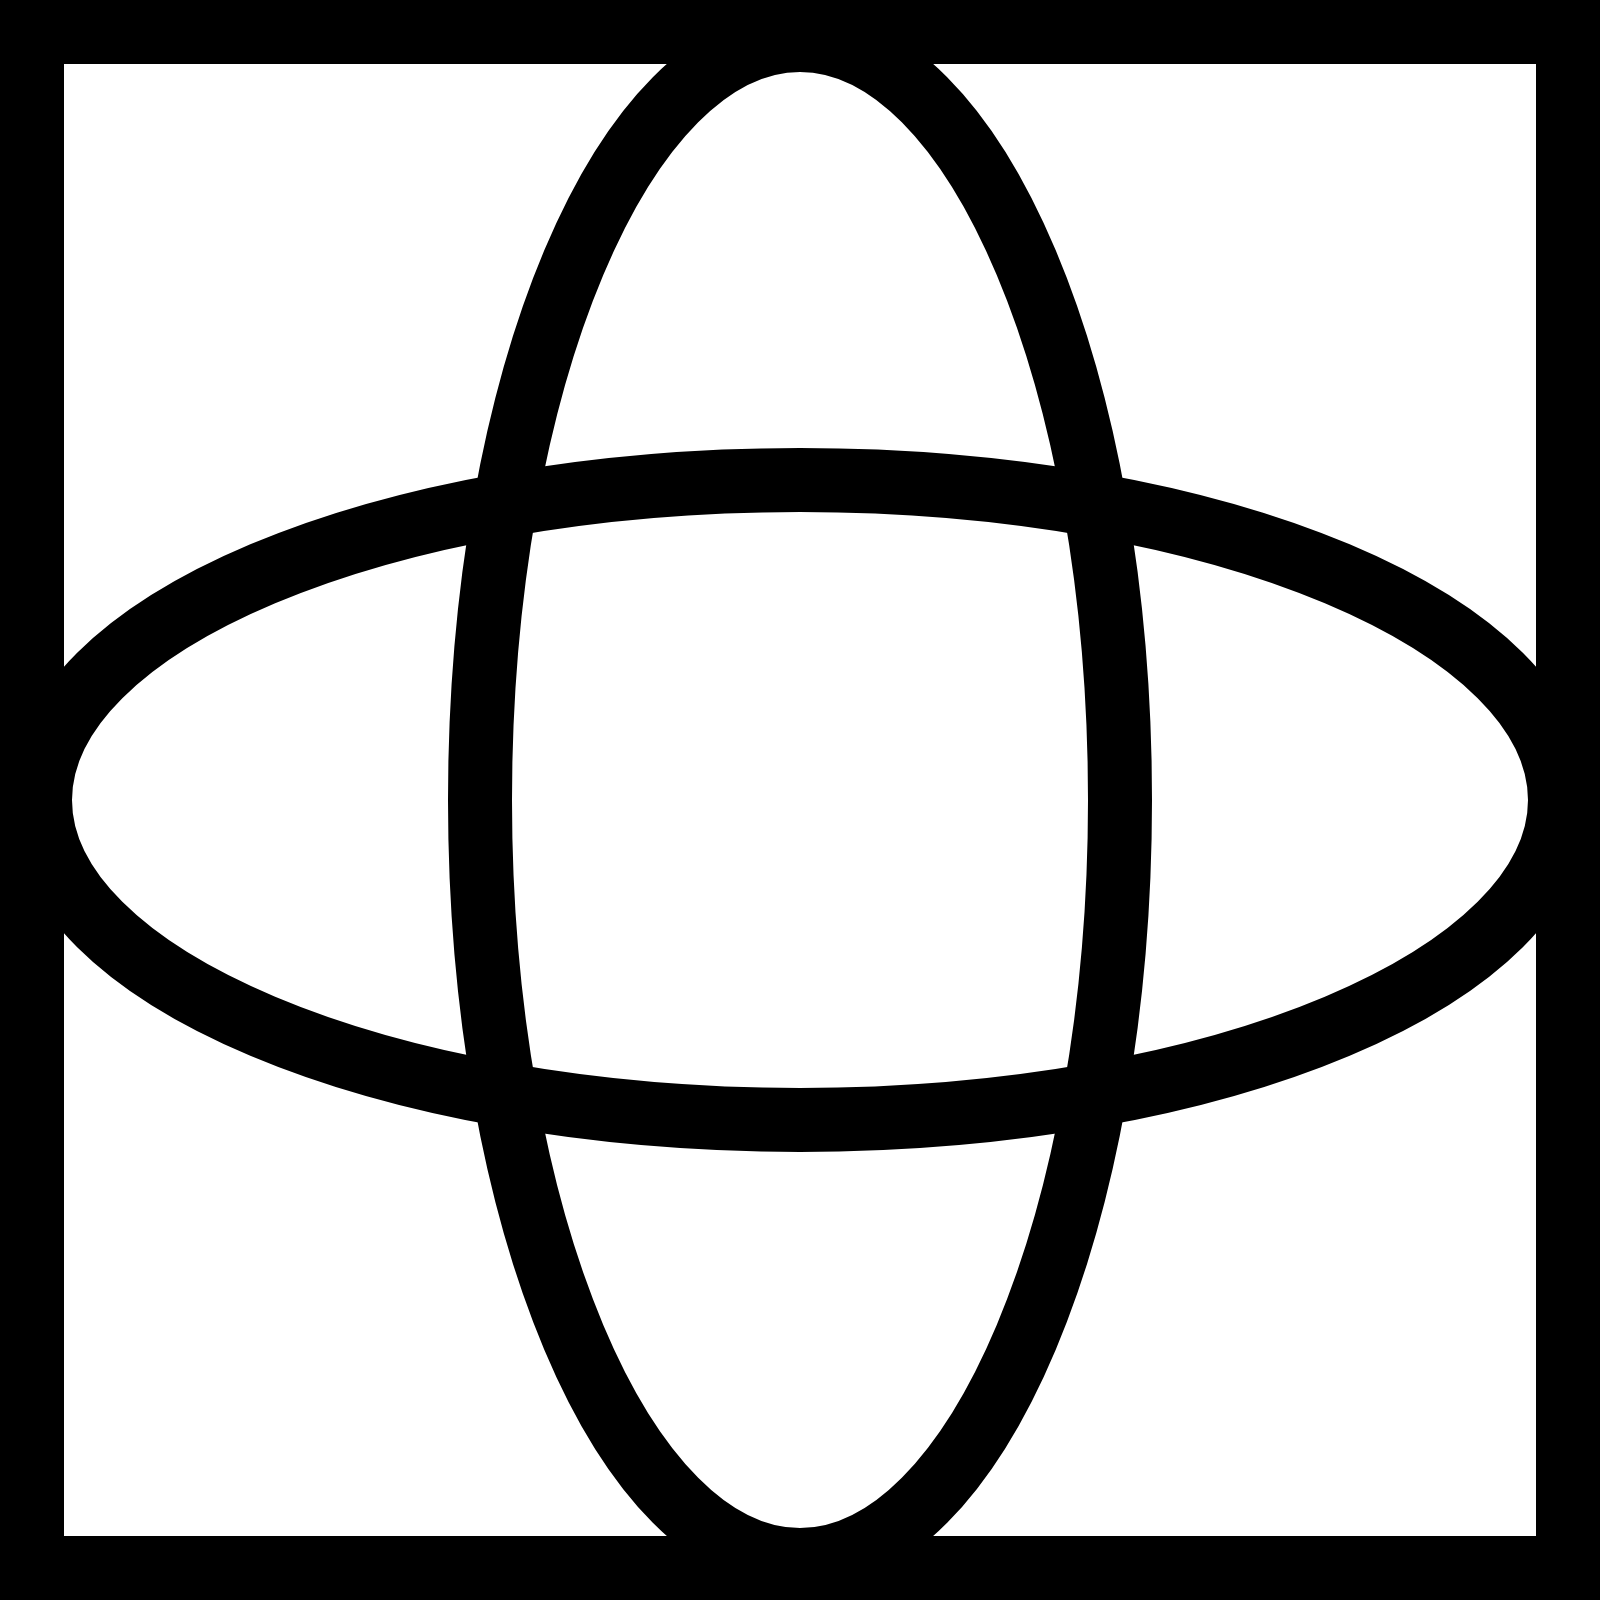
\includegraphics[width=300px]{img/empty-board.png}
    \caption[Prázdná herní plocha]{Prázdná herní plocha\footnotemark}
    \label{fig:empty-board}
\end{figure}

\footnotetext{všechny obrázky v práci jsou vlastní
práce autora, v případě herních ploch se jedná o snímky obrazovky z webové
aplikace popsané níže}

TickoaTTwo proti sobě hrají dva hráči, kteří se střídají v~tazích. Jeden hráč
na políčka v~hrací ploše kreslí svislé čáry, druhý hráč vodorovné čáry. Na
každé políčko může daný hráč hrát pouze jednou, avšak lze hrát na políčko, na
které už hrál protihráč. Nelze však hrát na políčko, na které hrál protihráč
v~jeho posledním tahu.

Není dáno, který hráč začíná.

Cílem každého hráče je dokončit řadu, sloupec či diagonálu, do které už hráli
oba dva hráči. Hra tedy končí ve stavu, kdy na hrací ploše je alespoň jedna
řada, sloupec či diagonála, ve které jsou tři \enquote{téčka}/\enquote{pluska}
(svislá čára od jednoho hráče, vodorovná čára od druhého hráče), podle toho i
stylizovaný název hry se třemi velkými písmeny~T.


% počet her: na každém políčku čtyři, to však děleno 4 protože 4 rotace
% nejkratší hra 6 tahů vyhrává druhý, u klasických 5 tahů vyhrává první
% WRONG nejrychlejší hra 15 (? pět T, 4 samostatné, patnáctý ukončí), u klasických 9

\section{Optimální strategie}
Zatímco klasické 3x3 piškvorky vždy končí remízou pokud hrají oba dva hráči optimálně
\cite{crowley1993}, tak u~TickoaTTwo nelze končit remízou. Budou-li oba hráči hrát
optimálně, vyhrává druhý hráč. Základním pravidlem je nevytvořit tři vlastní
znaky v~jedné vertikále/horizontále/diagonále, protože tím bychom dali
protihráči možnost je jednoduše doplnit a vyhrát. Nejhorší herní políčko je
tedy to prostřední, protože se v~něm protínají hned čtyři
vertikály/horizontály/diagonály (na rozdíl od klasických piškvorek, kde
prostřední políčko je jedno z~nejvíce žádaných \cite{xkcd832})

Optimální strategie pro druhého hráče je co nejdéle hrát naproti prvnímu hráči.
Jelikož první hráč nechce zabrat tři sousední políčka nebo hrát doprostřed, hra
se dostane do stavu, kde je šest políček plně zaplněno, uprostřed je jedna
volná diagonála a na tahu je první hráč, viz obrázek \ref{fig:empty-diagonal}

\begin{figure}[h]
    \centering
    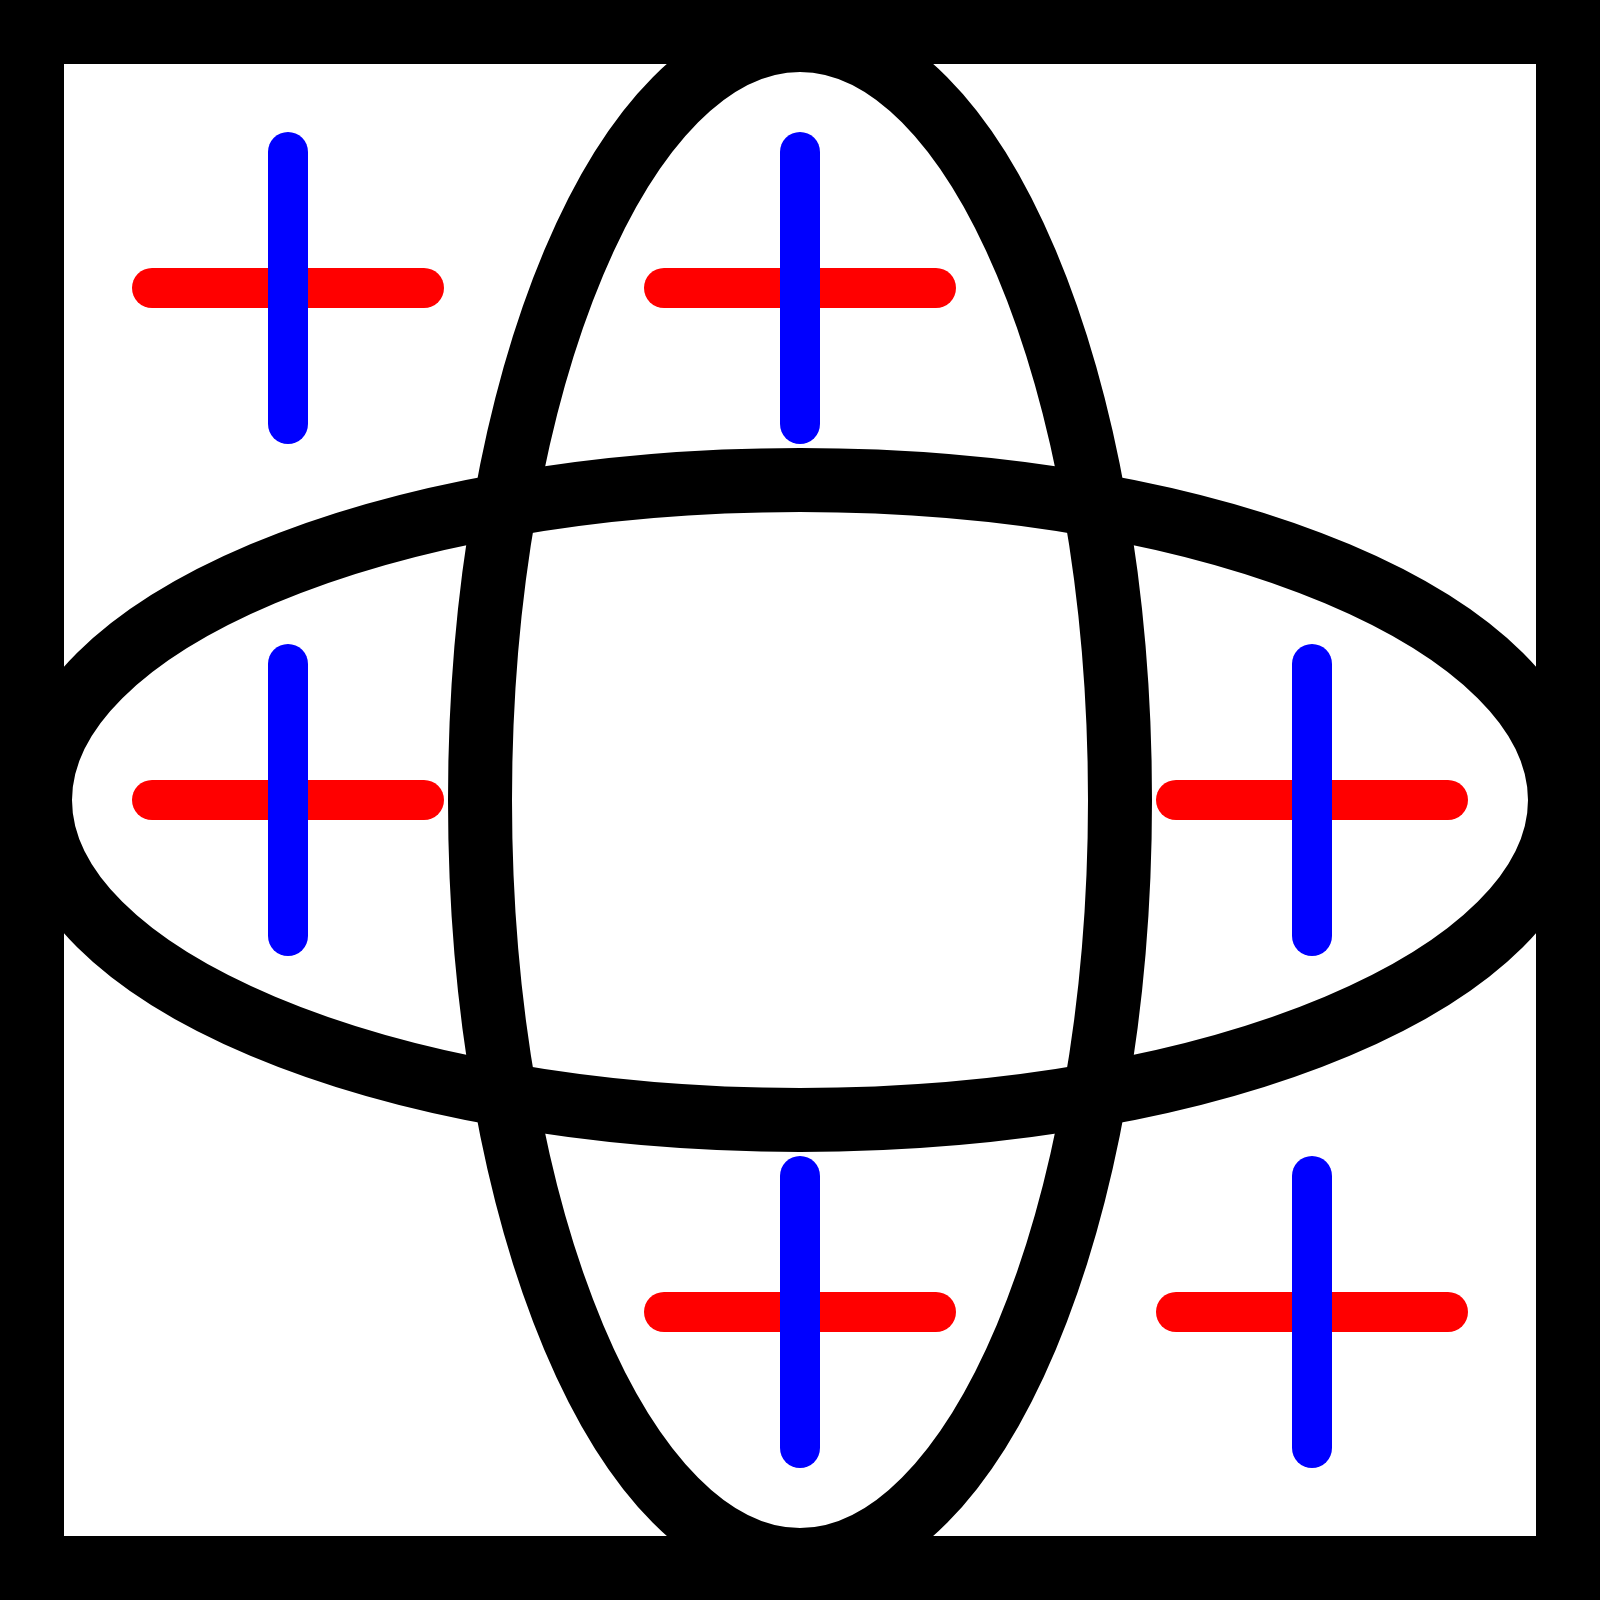
\includegraphics[width=300px]{img/empty-diagonal.png}
    \caption{Hra po devíti tazích optimální strategie}
    \label{fig:empty-diagonal}
\end{figure}

Ať zahraje první hráč kamkoli, druhý hráč bude hrát na další volné políčko
v~diagonále. První hráč následně zabere třetí volné políčko (jedno už zabral on,
na druhé hrát nemůže, protože ho zabral protihráč v~právě předchozím tahu).
Druhému hráč už tak pouze zbývá jedno jediné políčko, na které může hrát, které
ho dovede k~vítězství, viz obrázek \ref{fig:last-diagonal}.

\begin{figure}[h]
    \centering
    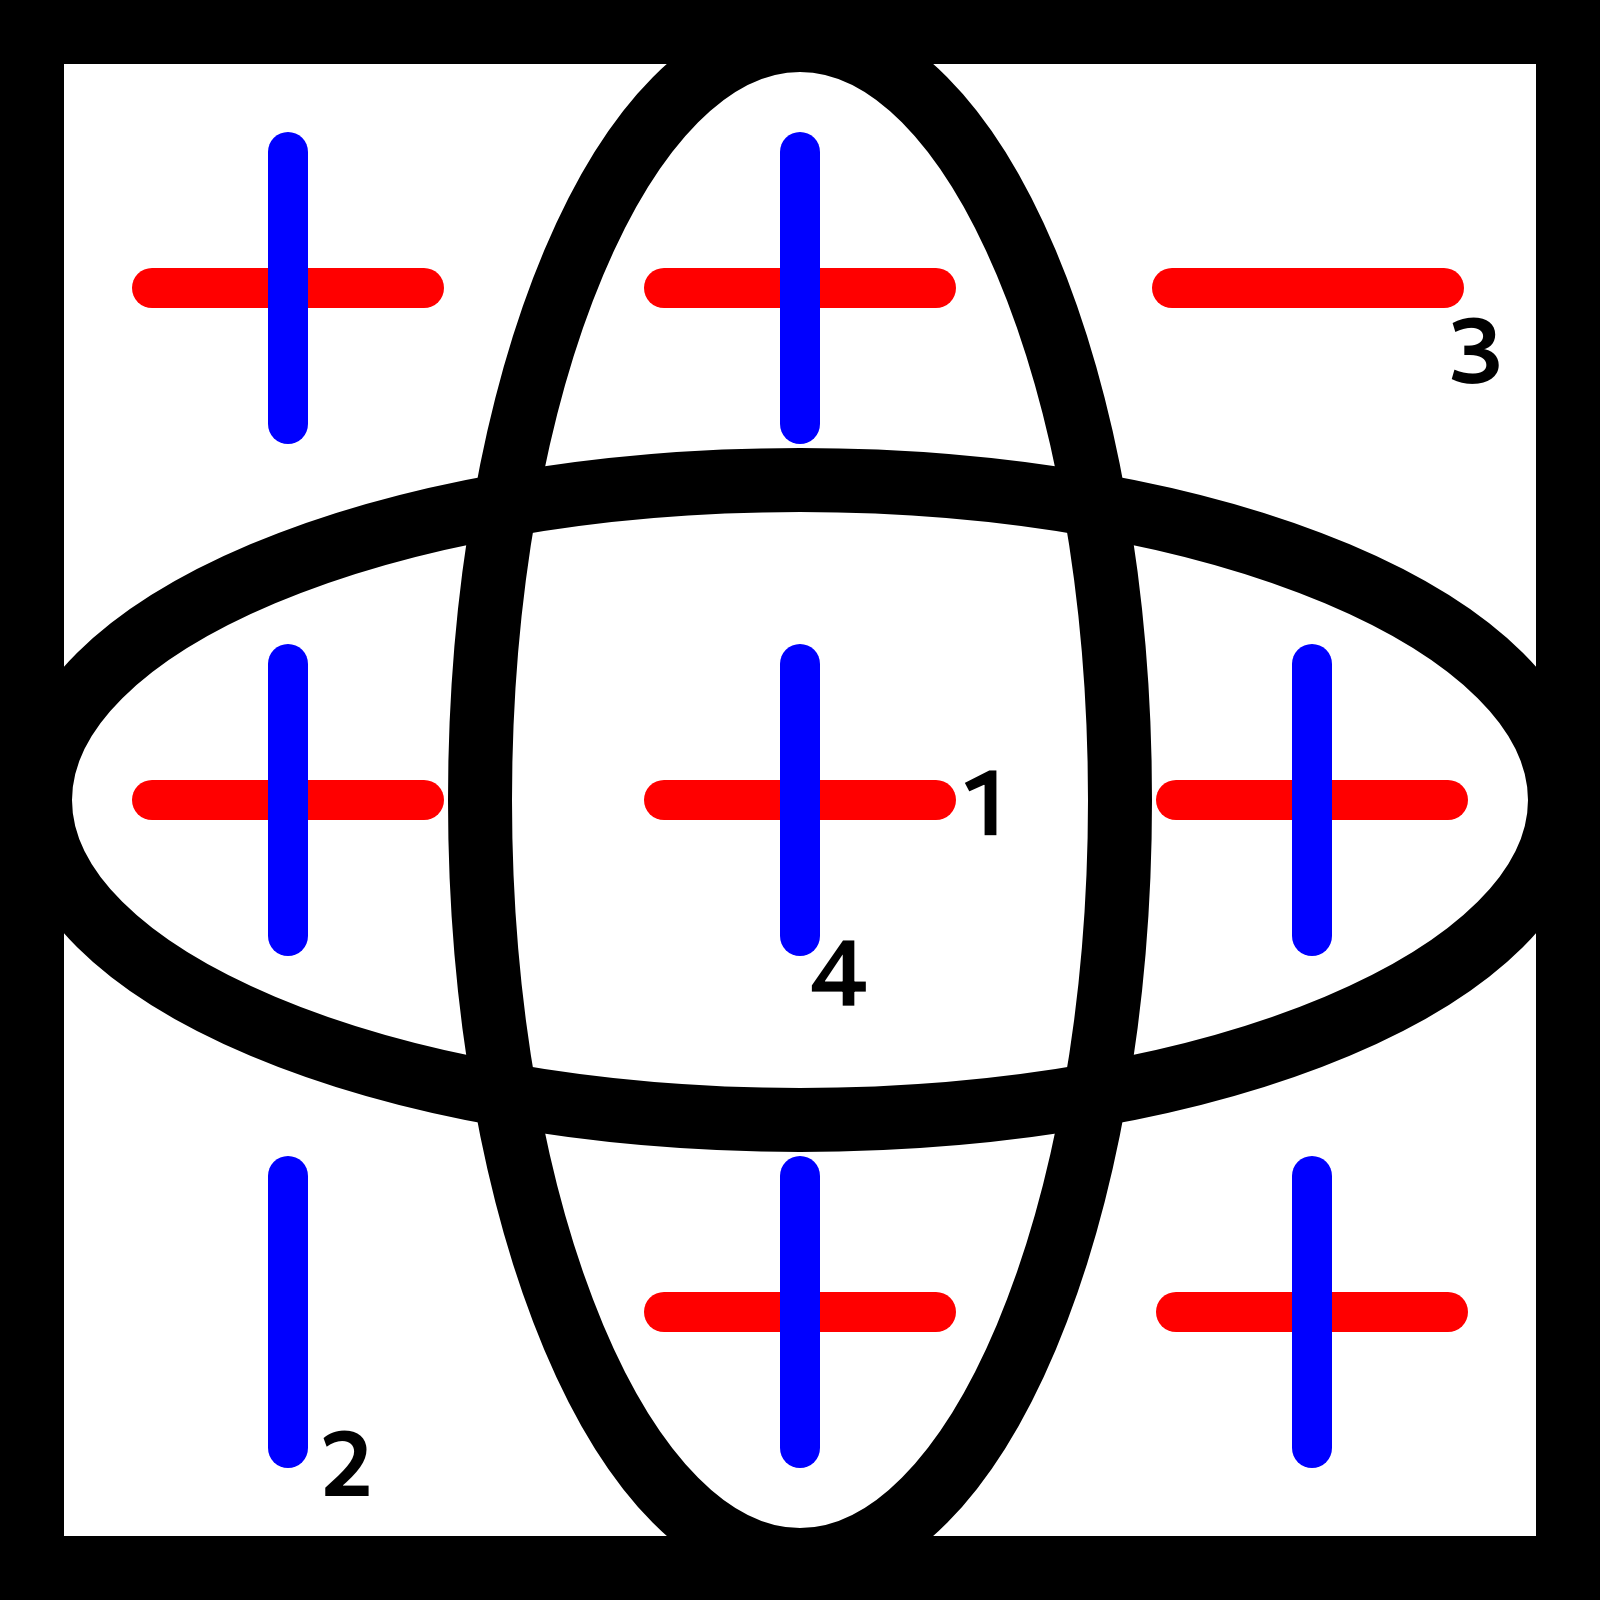
\includegraphics[width=300px]{img/last-diagonal.png}
    \caption{Možný průběh optimální hry pro poslední diagonálu, tahy očíslované}
    \label{fig:last-diagonal}
\end{figure}

\chapter{Vývoj implementace}

\section{Použité technologie}

Webová online multiplayer hra je implementovaná pomocí technologií, kterým se souhrnně říká T3 Stack. Podle oficiální dokumentace \parencite{t3stack} úkolem technologií T3 Stack je

\begin{enumerate}
    \item \B{Řešit problémy:} Neposkytovat všechny technologie, které jsou dostupné, ale poskytnout technologie, které jsou základem většiny webových aplikací a může být složité je nastavit manuálně.
    \item \B{\enquote{Krvácet} zodpovědně:} Poskytovat technologie, které jsou moderní a atraktivní, ale tak, aby v budoucnu netvořily problémy a případně se daly nahradit.
    \item \B{Typová bezpečnost není dobrovolná:} Znalost datových typů pomáhá programátorům s vývojem a bezpečným kódem, proto je v moderním vývoji naprosto nezbytná.
\end{enumerate}


Součástí T3 Stack je nástroj \M{create-t3-app}, který umožňuje vytvořit nový projekt, ve kterém jsou dané technologie předem nastavené.

Seznam technologií použitých:
\begin{itemize}
    \item \B{TypeScript:} Nadstavba nad programovacím jazykem JavaScript, která přidává typové anotace a jejich kontrolu. Tím umožňuje rychlejší a bezpečnější vývoj.
    \item \B{Next.js:} Moderní framework pro vytváření serverových částí webových  aplikací, slouží jako back-end pro React.
    \item \B{React:} Framework pro vytváření front-endových částí webových aplikací.
    \item \B{tRPC:} Knihovna pro bezpečnou a otypovanou komunikaci mezi front-endem (React) a back-endem (Next.js).
    \item \B{Prisma:} Knihovna pro komunikaci mezi back-endem (Next.js) a databází.
    \item \B{TailwindCSS:} Knihovna pro rychlé stylování webových aplikací.
\end{itemize}

Častou součástí této sady technologií též bývá NextAuth.js, které řeší přihlašování, registraci a správu uživatelů. Jelikož naše aplikace registraci uživatelů neumožňuje, není taková knihovna potřeba.

\section{Databáze}

Jako databáze k aplikaci byla zvolena PostgreSQL, jelikož se v dnešní době
jedná o jednu z nejpoužívanějších a nejoblíbenějších databází \cite{stackoverflow23}.

Schéma databáze je pouze jedna tabulka \M{GameSession} reprezentující jednu hru
mezi dvěma hráči. Vedle ní také enum \M{GridFieldState} reprezentující stav
jednoho hracího políčka (je prázdné, hrál na něj pouze první hráč, hrál na něj
pouze druhý hráč, hráli na něj oba hráči) a enum \M{GameState} reprezentující
stav hry (čeká se na druhého hráče, první hráč je na řadě, druhý hráč je na
řadě, první hráč vyhrál, druhý hráč vyhrál).

\begin{lstlisting}[language=Prisma]
enum GridFieldState {
    empty
    player1in
    player2in
    both
}

enum GameState {
    inviting
    player1plays
    player2plays
    player1won
    player2won
}

model GameSession {
    id          String      @id @default(cuid())
    createdAt   DateTime    @default(now())
    updatedAt   DateTime    @updatedAt
    slug        String      @unique
    player1     String?
    player2     String?
    visible     Boolean
    state       GameState   @default(inviting)
    lastPos     Int         @default(-1)
    grid        GridFieldState[]    @default([empty, empty, empty, empty, empty, empty, empty, empty, empty])
}
\end{lstlisting}




%%% Závěr
\chapter*{Závěr}
\addcontentsline{toc}{chapter}{Závěr}

Nově vzniklá hra TickoaTTwo má nyní implementaci, kterou si může kdokoli zahrát
s protihráčem online. Je dostupná na adrese \url{https://tickoattwo.mariansam.eu/}.
Zdrojový kód je zveřejněn pod MIT licencí na adrese
\url{https://github.com/mariansam/tickoattwo}, ten může sloužit nejen jako
referenční implementace hry TickoaTTwo, ale i jako příklad propojení tRPC
s~WebSockety.

Zároveň jsou sepsaná pravidla a vysvětlená optimální strategie, obojí může
sloužit jako základ pro další zkoumání této hry.

Věřím v~to, že se hra uchytí jako tradiční volba při večerech strávených
s~přáteli online, a i kdyby ne, snad si na ni občas někdo vzpomene alespoň jako
na \enquote{ten komický nápad, který někdo vzal vážně}.


\pagenumbering{gobble}
\newpage
\printbibliography[title=Literatura]
\nocite{*}
\addcontentsline{toc}{chapter}{Literatura}
\renewcommand{\baselinestretch}{1.5}

\lstlistoflistings
\addcontentsline{toc}{chapter}{Seznam programů}{\linespread{1}\selectfont}


\listoffigures
\addcontentsline{toc}{chapter}{Seznam obrázků}{\linespread{1}\selectfont}


\end{document}
